% Figure from MATH 591 notes, section 11. Compile with the notes preamble.
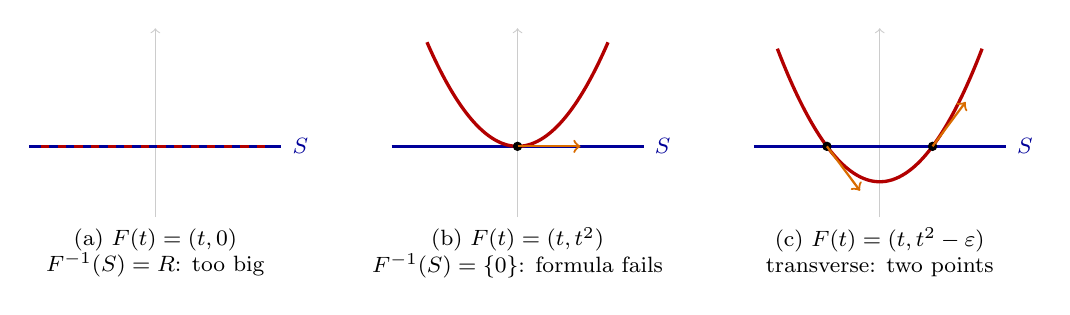
\begin{tikzpicture}[scale=1.0]
% ---- (a) curve lying in S
\draw[gray!40,->] (0,-0.9) -- (0,1.5);
\draw[blue!60!black,very thick] (-1.6,0) -- (1.6,0);
\draw[red!70!black,very thick,dashed] (-1.45,0) -- (1.45,0);
\node[blue!60!black,font=\footnotesize,anchor=west] at (1.62,0) {$S$};
\node[font=\footnotesize,align=center] at (0,-1.35) {(a) $F(t) = (t,0)$\\ $F^{-1}(S) = \mathbb{R}$: too big};
% ---- (b) tangent parabola
\begin{scope}[xshift=4.6cm]
\draw[gray!40,->] (0,-0.9) -- (0,1.5);
\draw[blue!60!black,very thick] (-1.6,0) -- (1.6,0);
\draw[red!70!black,very thick,domain=-1.15:1.15,samples=60,smooth,variable=\t] plot (\t,{\t*\t});
\fill[black] (0,0) circle (1.7pt);
\draw[orange!85!black,->,thick] (0,0) -- (0.8,0);
\node[blue!60!black,font=\footnotesize,anchor=west] at (1.62,0) {$S$};
\node[font=\footnotesize,align=center] at (0,-1.35) {(b) $F(t) = (t,t^2)$\\ $F^{-1}(S) = \{0\}$: formula fails};
\end{scope}
% ---- (c) perturbed, transverse
\begin{scope}[xshift=9.2cm]
\draw[gray!40,->] (0,-0.9) -- (0,1.5);
\draw[blue!60!black,very thick] (-1.6,0) -- (1.6,0);
\draw[red!70!black,very thick,domain=-1.3:1.3,samples=60,smooth,variable=\t] plot (\t,{\t*\t-0.45});
\fill[black] ({sqrt(0.45)},0) circle (1.7pt);
\fill[black] ({-sqrt(0.45)},0) circle (1.7pt);
\draw[orange!85!black,->,thick] ({sqrt(0.45)},0) -- ({sqrt(0.45)+0.42},{2*sqrt(0.45)*0.42});
\draw[orange!85!black,->,thick] ({-sqrt(0.45)},0) -- ({-sqrt(0.45)+0.42},{-2*sqrt(0.45)*0.42});
\node[blue!60!black,font=\footnotesize,anchor=west] at (1.62,0) {$S$};
\node[font=\footnotesize,align=center] at (0,-1.35) {(c) $F(t) = (t,t^2-\varepsilon)$\\ transverse: two points};
\end{scope}
\end{tikzpicture}
